\documentclass[final]{article}
\usepackage{txfonts}
\usepackage{palatino}
\usepackage[utf8]{inputenc}
\usepackage{authblk}
\usepackage{setspace}
\usepackage[margin=1.25in]{geometry}
\usepackage{graphicx}
\graphicspath{ {./figures/} }
\usepackage{subcaption}
\usepackage{amsmath}
\usepackage{optidef}

%%%%%% Bibliography %%%%%%
% Replace "sample" in the \addbibresource line below with the name of your .bib file.
\usepackage[style=authoryear-comp,
sorting=nty]{biblatex}
\addbibresource{references.bib}
\nocite{*}

%%%%%% Title %%%%%%
% Full titles can be a maximum of 200 characters, including spaces. 
% Title Format: Use title case, capitalizing the first letter of each word, except for certain small words, such as articles and short prepositions
\title{Factoring Consumer Staples}

%%%%%% Authors %%%%%%
% Authors should be listed in order of contribution to the paper, by first name, then middle initial (if any), followed by last name.
% Authors should be listed in the order in which they will appear in the published version if the manuscript is accepted. 
% Use an asterisk (*) to identify the corresponding author, and be sure to include that person’s e-mail address. Use symbols (in this order: †, ‡, §, ||, ¶, #, ††, ‡‡, etc.) for author notes, such as present addresses, “These authors contributed equally to this work” notations, and similar information.
% You can include group authors, but please include a list of the actual authors (the group members) in the Supplementary Materials.

\author[$\dag$]{Kyle Walsh}
\author[$\ddag$]{Siddharth Kantamneni}

%%%%%% Affiliations %%%%%%
\affil[$\dag$]{\small kew96@cornell.edu}
\affil[$\ddag$]{\small skk82@cornell.edu}

%%%%%% Date %%%%%%
% Date is optional
\date{}

%%%%%% Spacing %%%%%%
% Use paragraph spacing of 1.5 or 2 (for double spacing, use command \doublespacing)
\doublespacing

\begin{document}

\maketitle

%%%%%% Abstract %%%%%%
\begin{abstract}
\hspace{\parindent}In this paper, we attempt to determine if the Fama-French 3-Factor Model can be used with Markowitz Portfolio Optimization on the Consumer Staples sector. The Fama-French model is typically applied to the broader market, and we wanted to explore Consumer Staples because of the market crash due to the global pandemic. We implemented a Weighted Least Squares regressor to calculate assets' factor loadings and Markowitz Optimization for selecting maximum Sharpe Ratio portfolios. While this framework does achieve positive excess returns over the past fifteen years, the volatility makes it difficult to add to any portfolio. Sensitivity analysis did provide some insight into how parameters affect the model but further testing is required. Achieving a positive excess return gives us hope for this framework but necessitates future research into new factors and different techniques for calculating factor loadings.

\end{abstract}

%%%%%% Main Text %%%%%%

\section{Introduction}

\subsection{Motivation}
\hspace{\parindent} This project has been motivated by a desire to replicate the famed Fama-French Three-Factor model in a novel way. Wanting to stay consistent with the original theory, we decided to use the Consumer Staples sector as the entire universe, along with a risk-free asset. This allowed us to implement the original model with unknown outcomes.

Additionally, we wanted to see if the predictions from the model could be used to create portfolios with excess returns relative to the risk-free rate. If the model was truly able to predict excess returns, then one could ostensibly find sources of alpha among the consumer staples sector. Moreover, if our model was unable to do so, it may motivate finding additional or superseding factors to make the model more robust.

\subsection{Background}
\hspace{\parindent}Factor models are an extremely popular and rigorously explored investment model. Factor models seek to explain a stock's excess returns relative to a risk-free rate by computing coefficients based on the return of external "factors" which can vary widely. In general, there are two types of factor models: macroeconomic and fundamental. Macroeconomic models rely on factors that typically reflect the broader state of the economy. On the other hand, fundamental models use measurements that are specific to individual companies. 

\subsubsection{The Capital Asset Pricing Model}
\hspace{\parindent}Proposed in 1972 by Dr. Fischer Black, The Capital Asset Pricing Model (CAPM) was one of the first factor models. As a macroeconomic model, CAPM relies on a univariate regression of an asset's excess return on the market excess return, both over a risk-free interest rate. This method would pave the way for further using linear regressions to decompose the excess returns of various assets.

\begin{equation}
    \mathbb{E}\left[R_i\right]=r_f+\beta_i\left(\mathbb{E}\left[R_m\right]-r_f\right)
\end{equation}

As the "market factor", $\mathbb{E}\left[R_m\right]-r_f$ provides a general opinion on market direction. While $\beta_i$ is the regression coefficient on the market's excess return, it also represents an asset's market sensitivity. Often times, $\beta_i$ is referred to as a factor loading.

\begin{equation}
    \beta_i=\frac{Cov\left(R_i,R_m\right)}{Var\left(R_m\right)}
\end{equation}

\subsubsection{Fama-French Three-Factor Model}
\hspace{\parindent}Following the intuition of Black, in 1992, Dr. Eugene Fama and Dr. Kenneth French proposed an updated factor model, hoping to have more explanatory power when comparing to an asset's excess return. In addition to the market's excess return, Fama and French used two additional factors to represent a company's size and value. A company's market capitalization is often used as a facsimile for size. On the other hand, the book-to-market ratio often represents the value of a company, although other measures are able to be substituted, accordingly. These factors were chosen due to the phenomenon that small businesses tended to outperform large businesses and that value stocks (i.e. high book-to-market) would outperform growth stocks (low book-to-market).

As neither size nor value actually represent an asset's return, Fama-French proposed ranking the companies according to these measures - small to large for size and high to low for value. They then took the returns of the top assets and subtracted the returns of the bottom assets. These return-differences are now referred to as SMB (small minus big) for the size factor, and HML (high minus low) for the value factor. This model is a macroeconomic model because we use the market return on HML and SMB instead of the specific values of capitalization or book-to-market for each company.

\section{Methodology}

\subsection{Assumptions}
\hspace{\parindent}Assumptions underlying the Fama-French Three-Factor Model are all assumed to hold here. This includes the assumptions underlying linear regression. We also assume no trading costs, infinite liquidity/fractional trading, and no price impacts.

\subsection{Data}
\hspace{\parindent}The data was mainly collected from the Wharton Research Database Services (WRDS) along with investing.com. Within WRDS, the data was sourced from The Center for Research in Security Prices (CRSP) and Compustat.

\subsubsection{Investment Universe}
\hspace{\parindent}We started by including all current stocks in the S\&P 500 Consumer Staples sector. Due to the limited size of this set, and to avoid look-ahead bias on assets that entered into the S\&P 500's Consumer Staples during our timeline, we further pulled the six largest consumer staples focused ETFs' holdings over our timeline and added all stocks to the universe. In total, we generated 602 unique tickers which reduced to 350 after collecting the required data and eliminating those for which we did not have data points in each of the data sets. Many of these lost tickers represent other assets that are not classified as equities and, therefore, do not fit the parameters for our model.

\subsubsection{Cleaning}
\hspace{\parindent}As with most quantitative projects, the data cleaning process was much more involved than we hoped. While all data was collected from reputable sources, there was still substantial missing data for many companies in most of the required data fields. In general, missing data was handled with simplistic methods with specifics covered in the remaining paragraphs of this section. Furthermore, we only imputed a maximum of two periods (six months) of missing data as our investment universe is large enough to afford excluding incorrigible assets from consideration.

Although consistent adjusted-returns were provided for most assets, we still had to impute share price for many assets over our period in order to calculate the market capitalization of each company. For this data we assumed linearity for all missing points, including at the end of a period, and imputed accordingly.

For the same reason, we also had to impute missing shares outstanding. Unlike with prices, shares outstanding seems to remain constant over most time periods. For this reason, we used the most recent, previous shares outstanding. We only used back-looking data points because we make the assumption that the database will be updated whenever the number of shares outstanding is changed in either direction.

\subsubsection{Factors}
\hspace{\parindent} After cleaning the data, the factors were computed. To create the market excess factor, we subtracted the 3-Month US T-Bill (assumed to be our risk free rate) from the S\&P 500 Consumer Staples Index. Since our focus was on this Sector, we rationalized that we should have our factors be restricted to this sector as well. For computing the SMB factor, we computed the average returns of stocks that were either in the lower 10\textsuperscript{th} percentile or upper 90\textsuperscript{th} percentile in terms of market capitalization, and subtracted the average return of the 90\textsuperscript{th} percentile stocks from that of the 10\textsuperscript{th} percentile stocks, achieving our Small Minus Big "return." This process was repeated for every date in our data set. For HML we followed the same process, except we use the percentiles of book-to-market ratio instead of market capitalization and subtracted the average return of the 10\textsuperscript{th} percentile stocks from that of the 90\textsuperscript{th} percentile stocks. Once we had all of our factors computed, we were ready to start computing factor loadings for each stock.

\subsection{Computation of Model}
\hspace{\parindent}To ensure our model would not suffer from look-ahead bias, we chose to compute factors at every date beginning in 2005 Q1. We would only use data up to the period prior to the current period to compute the factor loadings for each stock. This simulates the model updating with the most up-to-date data at each period, further increasing model accuracy.

Actual computation of the factors utilized Weighted-Least-Squares (WLS) using a linear weighting system, with recent data being given the most weight. We then compared the excess returns of the stock in question against each of the factors using the WLS regression. This model returned our $\beta$ values, or factor loadings, for each of the factors and assets.

We now focused on calculating the alpha values for each asset, the portion of the expected excess return not explained by the model. There are two methods for obtaining this alpha value, which affected our model noticeably. One method includes a column of constants among the covariates of the WLS model, meaning that alpha serves as the intercept for the excess return of the assets. This method will be referred to as the "alternative model" in following sections. The other method does not include a constant in the covariates and calculates alpha as in Equation \ref{eq:3} and errors in Equation \ref{eq:4}. This second model will be referred to as the "base model" in subsequent sections due to its consistency with the theoretical model.

\begin{equation}
    \label{eq:3}
    \alpha_i := \Sigma_{t=1}^{T}w(t) *(r_{i}(t) - \Sigma_{j=1}^{m}\beta_{i,j}f_{j}(t))
\end{equation}

\begin{equation}
    \label{eq:4}
    e_{i}(t) = r_{i}(t)-\alpha_{i}-\Sigma_{j=1}^{m}\beta_{i,j}f_{j}(t)
\end{equation}

After computing the factor loadings and alpha, we must then compute the risk matrix for all of the stocks in a given time period. First, we must calculate the factor covariance matrix using Equation \ref{eq:5}. We then use Equation \ref{eq:6} to get the risk matrix where $\Delta$ is a diagonal matrix whose $i^{th}$ diagonal is $\Sigma_{t=1}^{T}w(t)e_i(t)^2$

\begin{equation}
\label{eq:5}
    F = \Sigma_{t=1}^{T}w(t)(f(t)-\Sigma_{s=1}^{T}w(s)f(s))(f(t)-\Sigma_{s=1}^{T}w(s)f(s))^{T}
\end{equation}

\begin{equation}
    \label{eq:6}
    V = BFB^T+\Delta
\end{equation}

\subsection{Markowitz Optimization}
\hspace{\parindent}In order to choose our optimal portfolio weights, we used Markowitz optimization techniques. As parameters for the objective function, we pass the expected excess returns and risk matrix we generated from the factor loadings in the previous section. These expected excess returns are first sorted, descending, according to expected return. We then only use the top and bottom $n/2$ returns (for a total of $n$ assets). As our objective function, we aim to maximize the portfolio's total expected return subject to a specified portfolio variance and market exposure. On top of these two common constraints, we also included constraints to ensure that we are not overexposed to any one asset by letting the maximum single position be one half of the total invested amount. These constraints further enforce that we only have long positions in the $n/2$ assets with the highest expected excess return and short the remaining assets. This model can be defined mathematically in Equation \ref{eq:7}.

\begin{equation}
\label{eq:7}
\begin{aligned}
& \underset{w}{\text{min.}}
& & \mu^T w \\
& \text{s.t.}
& & w^T V w\leq\sigma^2 \\
& & & e^T w=0 \\
& & & 0\leq w_i \leq 0.5
& & & & \forall i\in\{1,...,n/2\} \\
& & -&0.5\leq w_i \leq 0
& & & & \forall i\in\{n/2,...,n\} \\
\end{aligned}
\end{equation}

Our choice of being market neutral results from two initial findings. The first was that we noticed a strong inclination towards being long assets, effectively driving our short positions to be nearly zero while our long positions were nearly at the limit of their bounds. Along similar lines, by ensuring we are market neutral, we force the model to be more selective with our positions and eliminate any potential market drift that would be captured if we were long on average.

\section{Results}

\subsection{Performance}
\hspace{\parindent}As stated in section 2.3, we evaluated two models that differed only in the way that the alpha parameter is calculated. With a focus on following the original theory, we chose to use the method of calculating alpha using the results from WLS as our base model. For completeness, we have provided the results of both models with Table \ref{tab:1} containing the average values and Table \ref{tab:2} containing the standard deviations of the values from Table \ref{tab:1}.

\begin{table}[ht]
\parbox{0.5\linewidth} {
    \centering
    \begin{tabular}{|c||c|c|}
        \hline
         & \textbf{Base} & \textbf{Alternative}\\
         \hline\hline
        \textbf{Actual Return} & 4.76\% & 5.57\% \\
        \hline
        \textbf{Expected Return} & 33.07\% & 39.05\% \\
        \hline
        \textbf{Sharpe Ratio} & 0.34 & 0.35 \\
        \hline
    \end{tabular}
    \caption{Model metrics' expectations}
    \label{tab:1}
    }
    \hfill
\parbox{0.5\linewidth}{
    \centering
    \begin{tabular}{|c||c|c|}
        \hline
         & \textbf{Base} & \textbf{Alternative}\\
         \hline\hline
        \textbf{Actual Volatility} & 16.99\% & 18.67\% \\
        \hline
        \textbf{Expected Volatility} & 25.22\% & 24.45\% \\
        \hline
        \textbf{Sharpe Volatility} & 20.61\% & 20.50\% \\
        \hline
    \end{tabular}
    \caption{Model metrics' standard deviations}
    \label{tab:2}
    }
    \caption*{Note that "Return" refers to excess market return}
\end{table}

As we can see in Table \ref{tab:1} and Table \ref{tab:2}, while the alternative model does have a higher actual excess return, the base model performs only marginally worse than the alternative model. When comparing the excess returns over time in Figure \ref{fig:1}, we can see that they typically track well with each other over time, where the alternative model's higher volatility results from larger and more frequent excess return spikes.

\begin{figure}[ht]
    \centering
    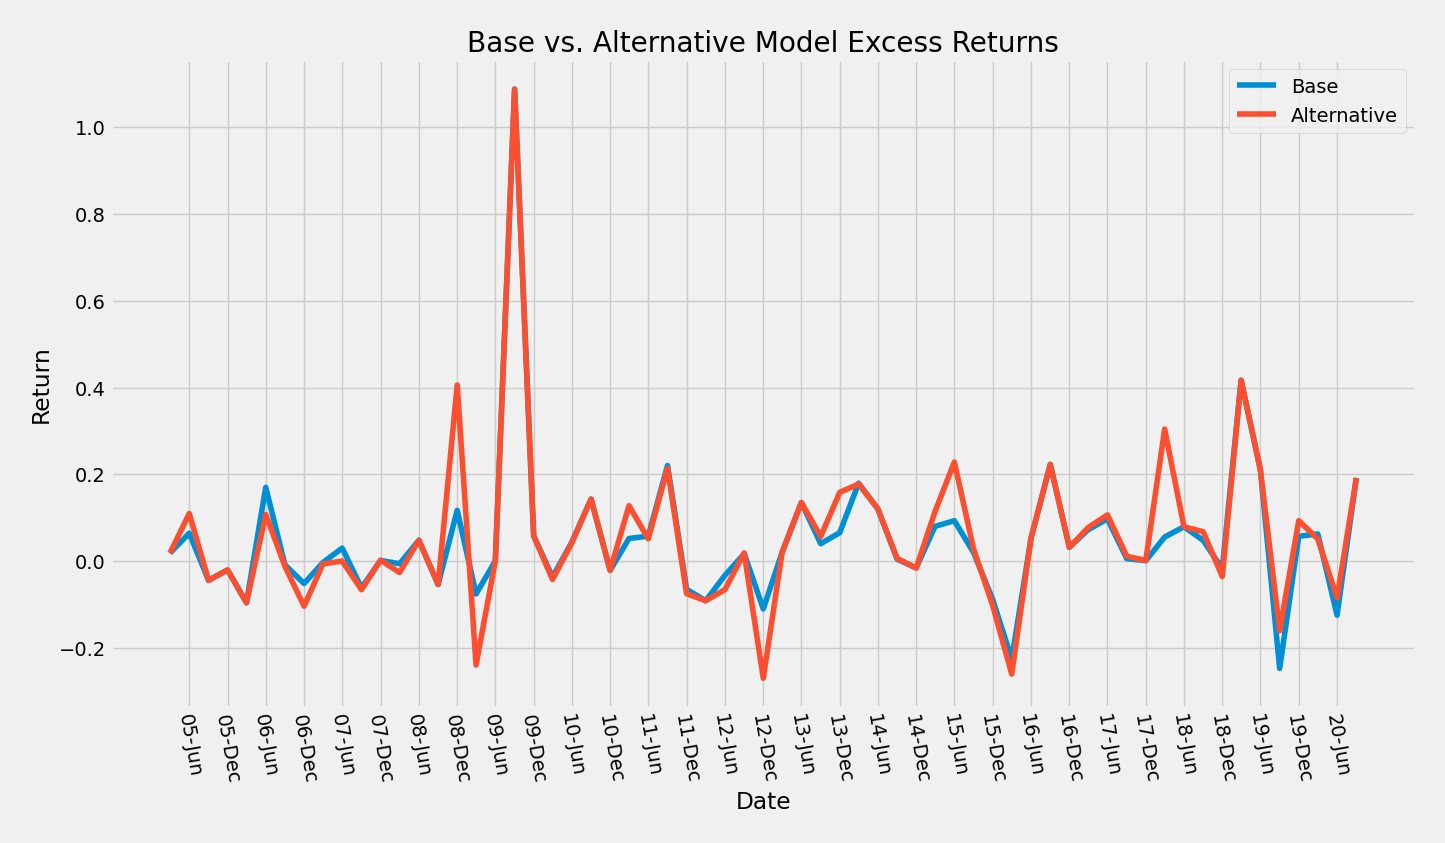
\includegraphics[width=1\textwidth]{base_vs_alternative_returns.png}
    \caption{Base and alternative model's actual excess return from 2005 through 2020}
    \label{fig:1}
\end{figure}

We now turn our attention to the base model. We can see in Figure \ref{fig:2} that the actual excess returns move relatively well with the expected excess return and this is represented by a correlation coefficient of 0.56. Unfortunately, the expected excess return given by the model is not representative of the excess return that will be achieved.

\begin{figure}[ht]
    \centering
    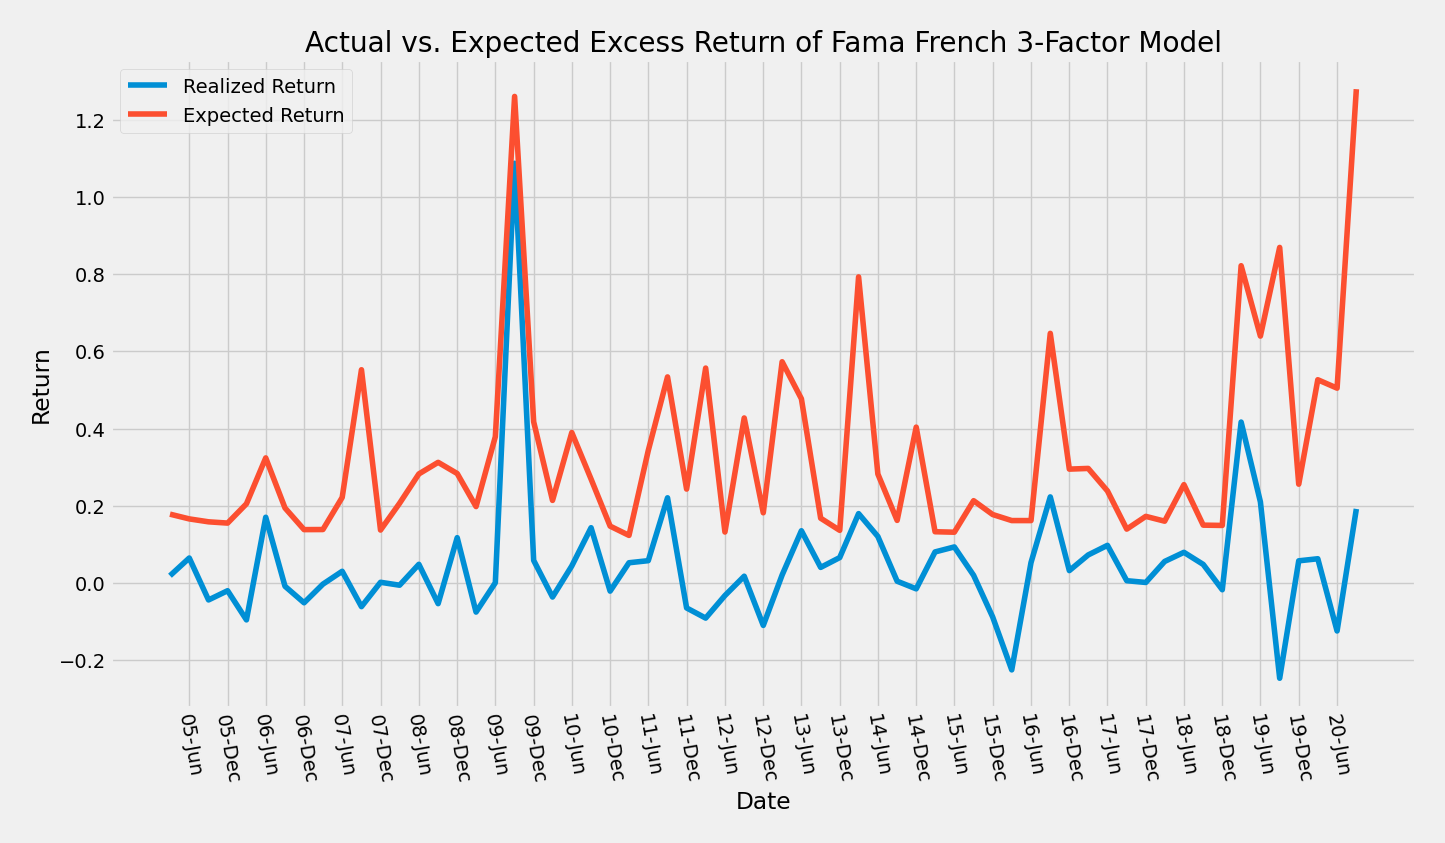
\includegraphics[width=1\textwidth]{actual_vs_expected_returns.png}
    \caption{Actual and expected excess return from 2005 through 2020}
    \label{fig:2}
\end{figure}

\subsection{Sensitivity Analysis}
\hspace{\parindent}In order to test our results against some variations in input assumptions, we performed a basic sensitivity analysis. We only looked at variations of two parameters: the basket size and the total market exposure. Overall, the results were promising on multiple fronts. When varying the basket size, we saw that too many or too few assets experienced reduced returns with an optimal size being between 10 and 50. On a similar note, when varying the market exposure, as we leave our neutral position, we see the portfolio experience higher excess returns with varying degrees of volatility. These results are summarized more concretely in Table \ref{tab:3} and Table \ref{tab:4} respectively.

\begin{table}[ht]
\parbox{0.5\linewidth} {
    \centering
    \begin{tabular}{|c||c|c|c|}
        \hline
         & \textbf{Return} & \textbf{Volatility}\\
         \hline\hline
        \textbf{4 Assets} & 5.34\% & 21.26\% \\
        \hline
        \textbf{10 Assets} & 6.51\% & 21.80\% \\
        \hline
        \textbf{20 Assets} & 4.76\% & 16.99\% \\
        \hline
        \textbf{50 Assets} & 6.26\% & 23.01\% \\
        \hline
        \textbf{100 Assets} & 5.07\% & 24.71\% \\
        \hline
    \end{tabular}
    \caption{Basket size}
    \label{tab:3}
    }
    \hfill
\parbox{0.5\linewidth}{
    \centering
    \begin{tabular}{|c||c|c|c|}
        \hline
         & \textbf{Return} & \textbf{Volatility} \\
         \hline\hline
        \textbf{-1.0 Exposure} & 8.66\% & 32.57\% \\
        \hline
        \textbf{-0.5 Exposure} & 7.57\% & 23.56\% \\
        \hline
        \textbf{0.0 Exposure} & 4.76\% & 16.99\% \\
        \hline
        \textbf{0.5 Exposure} & 6.70\% & 28.21\% \\
        \hline
        \textbf{1.0 Exposure} & 10.68\% & 34.26\% \\
        \hline
    \end{tabular}
    \caption{Market exposure}
    \label{tab:4}
    }
    \caption*{Note that "Return" refers to excess market return}
\end{table}

\section{Conclusion}

\hspace{\parindent}The Fama French 3 Factor Model, when employed in conjunction with Markowitz Optimization, shows potential for being able to create baskets of stocks with excess returns on a quarterly basis. Interestingly, when using the alternative model (where alpha is computed inside the linear regression) returns and risk are marginally higher and lower respectively. Obviously, the Sharpe Ratio and underlying risk of said portfolios are not suitable enough to warrant investing in such a strategy at this time. However, this could mean that assumptions underlying the calculation of alpha may not hold as the two portfolios are not the same. Ultimately, even with the predictions from the Fama French model, our Markowitz optimizer was unable to produce consistent results. This may be due to several confounding features. Firstly, the assumptions underlying the linear relationship between factors and excess return may not hold in the Consumer Staples sector. Secondly, our method of creating factor returns could have been erroneous, thus producing incorrect factors at each time period. Lastly, the errors of each model may not have had 0 expectation, resulting in heavily biased models.

\section{Future Research} 
\hspace{\parindent}Exploration into other factors such as momentum and profitability could prove insightful, especially since Fama and French themselves created models using those factors. We would also like to measure the effect of other economic metrics such as unemployment rate and how these play into returns in the Consumer Staples industry. In addition to traditional WLS, there are other regression and general machine learning techniques that could provide some improvement such as Bayesian Regression. Lastly, a dive into relaxing some of the assumptions in the models such as friction-less trading and infinite liquidity could allow us to the model into a more practical setting.

\clearpage

\printbibliography

\end{document}
